% ------------------------------------------------------------------------
% Documento auxiliar (standalone) do TCC
% Segurança da comunicação dongle <-> servidor
%
% Compilar a partir deste diretório (latex/aux-docs):
%   latexmk -pdf segunraca-dongle-server.tex
% Reutiliza a bibliografia e as figuras do documento principal (../).
% ------------------------------------------------------------------------
\documentclass[
	12pt,
	article,			% documento curto: sem capítulos nem página de rosto
	oneside,
	a4paper,
	english,
	brazil				% o último idioma é o principal do documento
	]{abntex2}

% ---
% Pacotes básicos (mesmos do main.tex)
% ---
\usepackage{lmodern}
\usepackage[T1]{fontenc}
\usepackage[utf8]{inputenc}
\usepackage{indentfirst}
\usepackage{color}
\usepackage{graphicx}
\usepackage{microtype}
\usepackage{longtable}
\usepackage{tikz}
\usepackage{amsmath}
\usepackage{float}

% Definição de cores para prioridades (mesmas do main.tex)
\definecolor{alta}{RGB}{200,0,0}
\definecolor{media}{RGB}{200,120,0}
\definecolor{baixa}{RGB}{0,140,0}

\newcommand{\palta}{\textcolor{alta}{\textbf{Alta}}}
\newcommand{\pmedia}{\textcolor{media}{\textbf{Média}}}
\newcommand{\pbaixa}{\textcolor{baixa}{\textbf{Baixa}}}

% ---
% Citações padrão ABNT
% ---
\usepackage[alf]{abntex2cite}

% Figuras do documento principal
\graphicspath{{../assets/}}

% ---
% Informações do documento
% ---
\titulo{Segurança da comunicação entre \textit{dongle} e servidor}

% ---
% Aparência do PDF
% ---
\definecolor{blue}{RGB}{41,5,195}
\makeatletter
\hypersetup{
	pdftitle={\@title},
	colorlinks=true,
	linkcolor=blue,
	citecolor=blue,
	filecolor=magenta,
	urlcolor=blue,
	bookmarksdepth=4
}
\makeatother

\begin{document}

\selectlanguage{brazil}
\frenchspacing

% Apenas o título (sem autor nem data)
\begin{center}
	{\Large\bfseries\imprimirtitulo\par}
\end{center}
\vspace{1em}

% ---
% Conteúdo
% ---
\textual

\section{Introdução} \label{sec:intro}

O propósito deste documento é modelar a implementação de uma comunicação com autenticidade entre
\textit{dongle} e um servidor externo, tendo como intermediário um \textit{app mobile} que se comunica com o 
\textit{dongle} por meio de \textit{BLE} e não pode ser confiado. Os dados devem trafegar 
para o servidor de modo que, ao recebê-los, deve ser criptograficamente garantido que eles foram 
medidos a partir do dongle que se identifica como originador do dado, a fim de que não seja 
possível alterar o conteúdo das medições ou deliberadamente esconder informação entre duas medições
diferentes sem que o servidor consiga detectar.

\section{Problemas a resolver} \label{sec:solucao}

O objetivo principal para o contexto deste trabalho é que as informações medidas pelo dongle que 
chegam no servidor possam ser confiadas e usadas para análises seguras a respeito do
funcionamento do carro e como ele está sendo conduzido. Assim, deve-se garantir autenticidade,
ou seja, todo registro recebido pelo servidor deve ter sido gerado pelo dongle associado a ele;
integridade, ou seja, o dado que é recebido pelo servidor não pode ter sido alterado; unicidade, 
ou seja, os registros devem ser apenas uma única vez e a ordem em que eles foram gerados deve
ser mantida; completude detectável, ou seja, o servidor deve saber exatamente se e quais registros
estão faltando ao sincronizar com o \textit{dongle}; e vínculo ao veículo, o que garante que o servidor
consigui identifica quando há troca de veículo entre os \textit{boots} do dongle.

Nesse contexto, só é poossível confiar plenamente no dongle e no servidor. Assim, o app e os enlaces BLE
e internet são modelados como não confiáveis, conforme a \autoref{fig:fronteiras-confianca}.

\begin{figure}[H]
	\centering
	\caption{Fronteiras de confiança entre \textit{dongle}, \textit{app} e servidor}
	\label{fig:fronteiras-confianca}
	% Fonte PlantUML: ../assets/aux-docs/plantuml/fronteiras-confianca.puml
	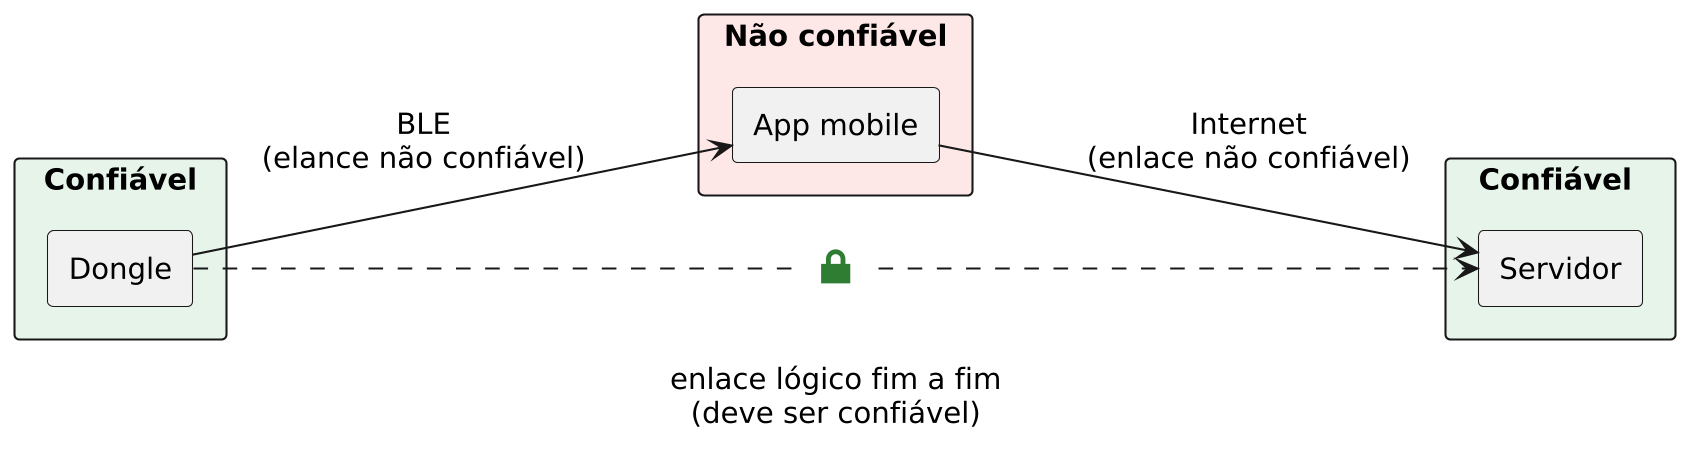
\includegraphics[width=\textwidth]{aux-docs/fronteiras-confianca.png}
	\legend{Fonte: elaborado pelo autor.}
\end{figure}


\subsection{Modelagem de ataques}

Existem diversos adversários e ataques que podem ser modelados cenário, envolvendo
os diferentes componentes e ligações entre eles. É possível dividir os ataques em quatro principais
categorias.

Dentro das categorias de ataque, também é possível definir 5 principais de adversários que aparecem entre elas:

\begin{itemize}
    \item (1) o terceiro perto de carro que pode ter acesso ao enlace de rádio do BLE, cujo objetivo é espionar ou injetar dados;
    \item (2) o próprio motorista que tem acesso ao app original do sistema, cujo objetivo é esconder, alterar medidas do dongle ou enviar as medidas do dongle para terceiros não autorizados;
    \item (3) um app de terceiro no celular pareado que pode acessar as características BLE, cujo objetivo é coletar as informações medidas para outros propósitos;
    \item (4) um atacante na rede entre o celular e o servidor, cujo objetivo é ler ou alterar dados no caminho para o servidor;
    \item (5) um invasor no servidor que tem acesso ao banco de dados e tudo que está armazenado, cujo objetivo pode ser apagar ou forjar dados.
\end{itemize}


Para especificar os ataques, será utilizada uma metodologia de modelagem que define o adversário, a pré-condição do ataque, o método 
a partir do qual o ataque é executado, a vulnerabilidade que ele explora, o alvo que está sendo atacado, e, por fim, o efeito que o ataque causa.


\subsubsection{Comunicação wireless no app}

Esses são ataques que se concetram tanto enlace BLE entre o app e dongle quanto na conexão de rede entre o app e o server. 
Dentre eles, estão sniffing, replay, Man In The Middle (MITM), acesso direto ao dongle por um terceiro e negação de serviço do enlace.

Abaixo estão modelados os ataques do ponto de vista do BLE, mas os mesmoes princípios podem ser pensados para um adverário do tipo (4) que interfere
na comunicação entre o app e o servidor.

Um exemplo de ataque dessa categoria é o sniffing (A1.1), no qual o adversário do tipo (1) pode querer obter os dados do motorista, afetando sua
privacidade. A pré-condição é ter um sniffer ao alcance do sinal do BLE, cujo enlace não é cifrado. O método a partir do qual ele é feito é
seguir a conexão e recuperar tudo que passa pelas características do dongle de maneira passiva. A vulnerabilidade explorada é a falta de cifração
nas características BLE, o alvo são os dados transferidos pelo enlace, e o efeito é o vazamento de dados medidos pelo dongle.

No ataque de \textit{replay} (A1.2), o adversário do tipo (1) quer repetir comandos ou respostas para alterar o estado do dongle ou enganar o app.
A pré-condição é ter capturado o tráfego por \textit{sniffing} e conseguir se conectar ao dongle ou se passar por ele. O método consiste em
reescrever na característica de recepção quadros gravados anteriormente, como \texttt{AT\#DIAG 1}, \texttt{AT\#PID} ou \texttt{ATZ}, ou em se
anunciar como o dongle e devolver respostas antigas ao app. A vulnerabilidade explorada é a ausência de autenticação da conexão e de
garantia de frescor das mensagens, somada ao fato de o app não verificar a identidade do dongle. O alvo são o modo e a configuração do dongle
e os dados exibidos pelo app, e o efeito é uma coleta pausada ou reconfigurada sem o conhecimento do motorista, ou um painel com valores falsos.

Já no \textit{Man In The Middle} (A1.3), o adversário do tipo (1) quer ler e alterar em tempo real o que app e dongle trocam. A pré-condição é estar
presente quando o app se conecta ou durante o pareamento, com dois rádios BLE. O método é conectar-se ao dongle, anunciar um clone dele ao
app e repassar todo o tráfego entre os dois, alterando valores ou inserindo comandos no caminho. A vulnerabilidade explorada é que nenhum dos
lados autentica o outro no enlace, o alvo é a integridade de comandos e respostas, incluindo as requisições ao barramento CAN no modo
diagnóstico, e o efeito é um painel adulterado e requisições injetadas no carro.

Por fim, no acesso direto (A1.4), o adversário do tipo (1) quer usar o dongle como se fosse o app. A pré-condição é que o dongle aceite conexões
de qualquer dispositivo, e o método é simplesmente conectar-se e escrever comandos na característica de recepção, inclusive requisições ao
barramento CAN no modo diagnóstico. A vulnerabilidade explorada é a falta de autenticação da conexão, agravada pelo dongle aceitar uma
segunda conexão simultânea. O alvo são os dados medidos, o modo diagnóstico e a configuração do dongle, e o efeito é a leitura dos dados,
a pausa da coleta e consultas ao veículo feitas em nome do dono.

Na negação de serviço do enlace (A1.5), o adversário do tipo (1) quer impedir que o app se comunique com o dongle, atacando a
disponibilidade da conexão. A pré-condição é estar ao alcance do sinal BLE do dongle. O método é conectar-se ao dongle assim que ele
começa a se anunciar e manter a conexão aberta, ocupando as conexões que ele aceita, de modo que o app oficial não consiga se conectar. 
A vulnerabilidade explorada é que o dongle aceita conexões de qualquer dispositivo e tem um número limitado delas. O alvo é a disponibilidade 
do enlace BLE e, por consequência, a sincronização dos registros com o servidor, e o efeito é um dongle inacessível ao app: o painel deixa de 
ser atualizado e o servidor recebe um intervalo sem dados que não é causado pelo motorista.

\subsubsection{Comunicação entre carro e dongle} \label{secsec:comunicacao-carro-dongle}

Já esses ataques acontecem no barramento CAN entre o carro e o dongle, ou seja, o atacante pode
usar algum elemento externo para simular a CAN do veículo por inteiro ou para sobrescrever um determinado PID a fim de
manipular leituras.

No ataque de ECU emulada (A2.1), o adversário do tipo (2) quer que a seguradora receba uma condução melhor do que a real. A pré-condição é ter
acesso físico à porta OBD e um emulador ou \textit{gateway} CAN, sendo que o próprio ECUSim deste projeto serve como prova de conceito.
O método é ligar o dongle no emulador, ou colocar um \textit{gateway} entre a porta e o dongle que repassa as requisições ao carro e altera
apenas as respostas escolhidas, como limitar a velocidade reportada. A vulnerabilidade explorada é que as respostas OBD-II não são
autenticadas, de modo que o dongle confia em quem responder. O alvo é a veracidade dos dados medidos antes de serem assinados, e o efeito
são registros autênticos com conteúdo falso: a assinatura prova que o dongle mediu, mas não que o carro disse aquilo.

Na resposta concorrente no barramento (A2.2), o adversário do tipo (2) quer sobrescrever apenas alguns PIDs sem retirar o carro do barramento.
A pré-condição é ter um dispositivo ligado ao CAN capaz de responder mais rápido que a ECU. O método é escutar as requisições funcionais,
enviadas para o identificador 0x7DF, e responder em 0x7E8 antes da ECU real. A vulnerabilidade explorada é a mesma do ataque anterior,
somada ao fato de o dongle aceitar a primeira resposta da faixa 0x7E8--0x7EF sem endereçar ECUs específicas. O alvo é a veracidade dos PIDs
escolhidos, e o efeito, além dos registros autênticos com conteúdo falso, é um painel e um diagnóstico enganados.

\subsubsection{App malicioso} \label{secsec:app-malicioso}

Como o aplicativo será instalado no aparelho do usuário do dongle, um aparelho com \textit{root} tem total controle do
funcionamento do app e pode manipulá-lo para gerar ataques ao sistema. Esses ataques podem manipular o processo de envio dos
dados entre o app e o servidor a fim de fazer com que as informações do servidor não correspondam com o que foi realmente medido 
pelo dongle no carro. O principal adversário nesse contexto é o do tipo (2), que controla o app e pode querer forjar cenários de
medição que vão de encontra aos interesses da entidade no servidor externo, como uma seguradora ou gerenciadora de frotas.

Na exfiltração (A3.1), o adversário do tipo (3), ou um SDK de terceiros embutido no próprio app, quer vender ou usar para outros fins os dados de
condução e de posição do motorista. A pré-condição é ter permissão de Bluetooth e de internet no celular pareado com o dongle. O método é
conectar-se ao dongle quando o app oficial não está conectado e ler os dados medidos, ou ler os registros e posições que passam pelo app,
enviando tudo a outro servidor. A vulnerabilidade explorada é que os dados não são cifrados na camada de aplicação e que a autorização é
feita por aparelho, e não por app. O alvo é a privacidade do motorista, e o efeito é o vazamento de dados pessoais e o rastreamento do veículo.

Na pausa da coleta (A3.2), o adversário do tipo (2), por meio de um app modificado, ou o do tipo (3), quer esconder trechos da direção. A pré-condição
é ter acesso às características BLE do dongle por um celular pareado, e o método é enviar \texttt{AT\#DIAG 1} antes de dirigir e
\texttt{AT\#DIAG 0} depois, tirando o dongle do modo de coleta durante o trajeto. A vulnerabilidade explorada é que a troca de modo não exige
autorização do servidor. O alvo é a completude da coleta, e o efeito é um intervalo sem dados que se parece com um uso legítimo do modo diagnóstico.

Já na omissão de mensagens do servidor (A3.3), o adversário do tipo (2), por meio de um app modificado, quer degradar a coleta sem que a culpa
recaia sobre o app. A pré-condição é que o app seja o único caminho entre o servidor e o dongle. O método é receber do servidor o desafio, a
confirmação de recebimento ou o \textit{token} de diagnóstico e não repassá-los ao dongle, ou repassar apenas alguns. A vulnerabilidade
explorada é que as mensagens do servidor não têm confirmação de entrega ao dongle. O alvo é a recuperabilidade dos registros, a âncora de
tempo e a troca de época, e o efeito é que, sem confirmações, a memória do dongle enche e ele descarta registros antigos; sem desafio, não
há âncora de tempo nem época nova; e, sem \textit{token}, o diagnóstico é negado.

Na alteração de medições (A3.4), o adversário do tipo (2) quer melhorar o próprio histórico. A pré-condição é controlar o app, ou um \textit{proxy}
com uma autoridade certificadora instalada no celular, e o método é modificar bytes de um bloco antes de enviá-lo ao servidor. A
vulnerabilidade explorada é a ausência de integridade fim a fim, o alvo é a integridade dos registros, e o efeito é a aceitação de dados falsos.

Na repetição de medições (A3.5), o adversário do tipo (2) quer repetir uma viagem tranquila. A pré-condição é ter gravado blocos antigos, e o método
é reenviar ao servidor blocos já aceitos. A vulnerabilidade explorada é a falta de garantia de unicidade, o alvo é a unicidade dos registros,
e o efeito são dados duplicados no servidor.

Na reordenação das medidas enviadas (A3.6), o adversário do tipo (2) quer deslocar eventos no tempo. A pré-condição é controlar o app, e o método é enviar os blocos
fora de ordem. A vulnerabilidade explorada é que a ordem dos registros não é garantida, o alvo é a ordem dos registros, e o efeito é uma
linha do tempo falsa.

No descarte de medições intermediários (A3.7), o adversário do tipo (2) quer apagar um evento específico, como uma frenagem brusca. A pré-condição
é controlar o app, e o método é deixar de enviar os blocos escolhidos. A vulnerabilidade explorada é a falta de completude, o alvo é a
completude dos registros, e o efeito é uma lacuna silenciosa nos dados do servidor.

Ao omitir as últimas medições (A3.8), o adversário do tipo (2) quer omitir a última viagem. A pré-condição é controlar o app, e o método é parar de enviar
blocos antes do último. A vulnerabilidade explorada é que o servidor não conhece o número de sequência do último registro gerado, o alvo é a
completude dos registros, e o efeito é uma perda de dados invisível ao servidor.

Ao parar de sincronizar propositalmente o dongle com o app (A3.9), o adversário do tipo (2) quer não reportar nada. A pré-condição é poder desligar o app ou o Bluetooth, e o método é
nunca abrir uma sessão com o servidor. Não há vulnerabilidade técnica a explorar, pois é impossível obrigar o app a sincronizar; o alvo é a
completude dos registros, e o efeito é a ausência de dados.

\subsection{Definição de escopo e mitigação de ataques}


Tendo em vista todos esses possíveis ataques, é necessário alinhar o escopo do projeto de acordo com o objeito que ele se propões a cumprir.
Como a ideia é fazer com que os dados cheguem no servidor de maneira confiável e completa, foram priorizados os ataques da categoria \ref{secsec:app-malicioso},
sendo o objetivo deste documento explicar em detalhe um protocolo que garante, nesse cenário de desconfiança no canal e no aplicativo que intermedia o envio dos dados,
como garantir autenticidade, integridade, unicidade e completude detectável dos dados medidos pelo dongle.

Fica como limitação do projeto a mitigação de ataques que envolvam o barramento CAN do veículo, como os da categoria \ref{secsec:comunicacao-carro-dongle},
pois o escopo do projeto envolve apenas os dados medidos pelo dongle, sem abordar a garantir de que o dongle está realmente conectado em uma rede CAN válida, o
que deve ser garantido externamente. Alguns exemplos de mitigação para isso é incoporar o dongle dentro da arquitetura do carro e não exposto na conexão OBD2 interna,
configurar alertas de desconexão para entender se o dongle foi retirado a fim de ser colocado em um simulador, ou cruzar a medida com sensores externos de velocidade e 
localização instalados externamente à rede CAN.


\subsection{Segurança na comunicação sem fio}



\postextual

\bibliography{../abntex2-modelo-references}

\end{document}
